\subsection{Node roles and task paths}
\label{section:roles}

%%%%%%%%%%%%%%%%%%%%%%%%%%%%%%%%%%%%%%%%%%%%
\newcommand{\formalAtomicTaskRole}[2]{
	\functionFormal{#1}
	{\setAtomicTaskInstance{}{} \times \setAgent{}{}}
	{ \setAgent{}{}}
}
\newcommand{\formalCompositeTaskRole}[2]{
	\functionFormal{#1}
	{\powerSetAtomicTaskInstance{}{} \times \setAgent{}{}}
	{ \setAgent{}{}}
}
\newcommand{\formalSinkRole}[2]{
	\formalCompositeTaskRole{sink}{}}
\newcommand{\formalDetectorRole}[2]{
	\formalAtomicTaskRole{detect}{}}
\newcommand{\formalRelayRole}[2]{
	\formalAtomicTaskRole{relay}{}}

\newcommand{\functionAtomicTaskRole}[2]{
	\functionSignature{#1}
	{\varAtomicTask{}{}, \varAgent{}{}}
}
\newcommand{\functionCompositeTaskRole}[2]{
	\functionSignature{#1}
	{\setAtomicTaskInstance{}{}, \varAgent{}{}}
}
\newcommand{\functionSinkRole}[2]{
	\functionCompositeTaskRole{sink}{}}
\newcommand{\functionDetectorRole}[2]{
	\functionAtomicTaskRole{detect}{}}
\newcommand{\functionRelayRole}[2]{
	\functionAtomicTaskRole{relay}{}}

\reviewquestion{What happens to the measurement, e.g. is it stored by the sensor node, or communicated by the sensor node directly out of the system, or back along the task-path to the sink node, or along a potentially different path to the sink node, or something else? While I know you go on to explain more detail in later sections, it seems odd to omit the end of the description of what happens to a request at this point.
}
\reviewquestion{Figure 2 seems inconsistent with the text early in the section.
	- How can there be nodes that are distinctly 'sensor nodes' when you say every node has 'one or more sensors'? When you say "...a final measurement is made by a sensor node" do you mean "a sensor node *for that task*", i.e. it is a role played for a given task rather than a distinct kind of node?  If it is meant to be a role within a task, 'sensor node' sounds like a type rather than a role, so there may be a better name to use.
	- When every node has an agent by your definition, then why are some elements in the figure called nodes and others (apparently of the same kind) called agents? 
}
\reviewquestionopen{Why does one agent (and possibly by implication other agents) have a 'broadcast radius of node' shown, but this broadcast radius is not mentioned as a property of an agent or node in the text?}


\reviewquestion{This is clearer than in Section 3.1, but the use of terms seems inconsistent again. In Section 3.1, nodes were hardware while agents were software. In Section 3.2, the terms were interchangeable. In Section 3.3, nodes are roles that agents can play with regard to an atomic task. This is too confusing - there needs to be some consistency.
}
\reviewquestion{The distinction between idle node and sleep node roles for an atomic task seems odd, as neither appears to have any part in the completion of the task. This is just a note not necessarily a point of concern - maybe the reason for distinguishing them becomes clearer later in the paper.
}
\reviewquestion{As said for Section 3.1, I still don't understand what happens to the measurement once it is taken.
}

For each atomic task, agents will have different \textit{roles} for that task,  what behaviours they take on to help complete the task. A \textit{sink} is an agent that  receives a set of tasks from outside the system, $\formalSinkRole{}{}$. A \textit{relay} is an agent that is allocated an atomic task, but does not complete it, instead re-allocating it to other agents, $\formalRelayRole{}{}$. A \textit{detector} is an agent that  executes an atomic task, and so performs the measurement, $\formalDetectorRole{}{}$.

The steps of a task completion are,

\begin{enumerate}
	\item A set of atomic tasks $\setAtomicTaskInstance{}{}$ is sent from an agent external to the system.
	\item  $\functionSinkRole{}{}$ can either complete each atomic task $
	\varAtomicTask{}{} \in \setAtomicTaskInstance{}{}$ itself, or allocate it to another agent.
	 \item $\functionRelayRole{}{}$ receives an atomic task, and passes it on to another agent.
	 \item $\functionDetectorRole{}{}$ performs the atomic task.
	 \item The detector returns the results of the atomic task execution back to the agent that allocated it $\varAtomicTask{}{}$.
	 \item Relay agents pass back the atomic task results to the agents that allocated the corresponding atomic task to them, until the results reach the initiating sink agent.
	 \item The sink agent aggregates the results of all the atomic tasks $ \varAtomicTask{}{} \in \setAtomicTaskInstance{}{}$ and sends this aggregated result back to the external agent that sent it the set of tasks $\setAtomicTaskInstance{}{}$.
\end{enumerate}

With these roles in mind, we can now define the  \textit{task-path} as a mapping of atomic tasks to ordered sequence of agents $\formalTaskArc{}{}$ that each atomic task $\varAtomicTask{}{}$ is sub-allocated to. The first agent is that of the sink node that has received the initial composite task, and the last agent is that of the sensor node that executes the atomic task, with the sequence of agents in-between those of the active nodes relaying the atomic task. So for a task path of depth $n$, we have
$\functionTaskArc{}{} = \lbrace \functionSinkRole{}{}, \functionRelayRole{i}{}, \functionDetectorRole{}{} \rbrace_{i=1}^{n-2}$. 


\begin{figure}
	\centering 
	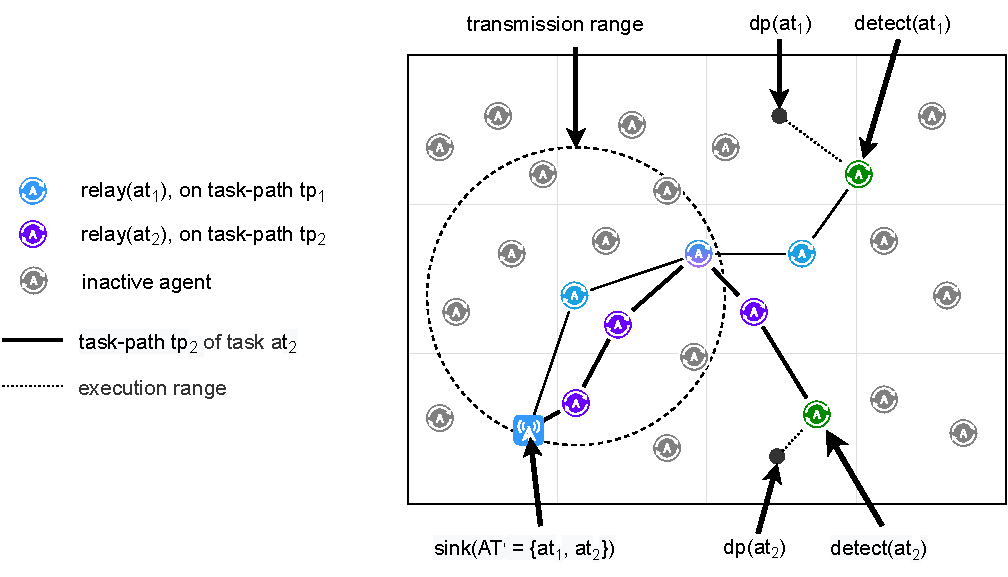
\includegraphics[width=0.9\linewidth, trim={25pt 0pt 24pt 0pt, clip}]{grid_concept}
	\caption[WSN deployment terminology]{WSN components and terminology}
	\label{fig:grid_concept}
\end{figure}


 These concepts are illustrated in Figure \ref{fig:grid_concept} and will be detailed in the following sections.

